% The `reedthesis' class (.cls) file has a number of options. Most of these
% options are passed directly to the book class, but we have a number of custom options:
% - `notocchapterdots' - disable the Table of Contents dots between chapters.
%	This only affects the dots between the Chapter N: ... heading and their respective page numbers.
% - `notocsectiondots' - disable the Table of Contents dots between section.
% - `tocchaptername=false' - shows just "N" instead of "Chapter N" in each ToC entry.
% - `headerstyle' - chooses the format in which header titles are displayed
%	- `headerstyle=uppercase' - displays header titles in upper case
%	- `headerstyle=smallcaps` - displays header titles in small caps.
% - `linkstyle' - changes the style of links. by default, this is "unstyled" (black)
%	(Note: If you go to print, and links don't show up, check your LaTeX engine! This should work fine on Overleaf, but you may need to
%		change which LaTeX engine you use (e.g. for LaTeX Workshop on Visual Studio Code, use the recipe `pdflatex'))
%   - `linkstyle=web` - the color of a link is always blue ("website"-style)
% 	- `linkstyle=labelled` - the color of a link depends on its type
% - `bibstyle` - choose the bibliography style in use. defaults to numeric
% - `bibfile=???.bib' - the name of the bibliography file. defaults to bibliography.bib
\documentclass[
	12pt,
    twoside,
    bibstyle=ieee,
    bibfile=bibliography.bib,
    headerstyle=uppercase,
]{reedthesis}
\usepackage{graphicx,latexsym} 
\usepackage{amssymb,amsthm,amsmath}
\usepackage{longtable,booktabs,setspace} 
\usepackage{rotating} 
\usepackage[english]{babel}


\title{Undefined Thesis Paper Project}
\author{Riley Wood}
\date{May 2026}
\division{Mathematical and Natural Sciences}
\advisor{Greg Anderson}
\altadvisor{Ang\'elica Osorno}
\department{TBD}
% if you're writing a thesis in an interdisciplinary major,
% uncomment the line below and change the text as appropriate.
% check the Senior Handbook if unsure.
%\thedivisionof{The Established Interdisciplinary Committee for}
% if you want the approval page to say "Approved for the Committee",
% uncomment the next line
%\approvedforthe{Committee}

\setlength{\parskip}{0pt}



\begin{document}

  \maketitle
  \frontmatter % this stuff will be roman-numbered
  \pagestyle{empty} % this removes page numbers from the frontmatter


% Acknowledgements (Acceptable American spelling) are optional
% So are Acknowledgments (proper English spelling)
%    \chapter*{Acknowledgements}
%	I want to thank a few people.


% The preface is optional
%    \chapter*{Preface}
    \tableofcontents
% if you want a list of tables or figures, optional
%    \listoftables
%    \listoffigures

%   % If your abstract is longer than a page, there may be a formatting issue.
    \chapter*{Abstract}
	The preface pretty much says it all.
	

%   
	\chapter*{Dedication}
	You can have a dedication here if you wish.



  \mainmatter % here the regular arabic numbering starts
  \pagestyle{fancyplain} % turns page numbering back on
  
%The \introduction command is provided as a convenience.
%if you want special chapter formatting, you'll probably want to avoid using it altogether

    \chapter*{Introduction}
         \addcontentsline{toc}{chapter}{Introduction}
	\chaptermark{Introduction}
	\markboth{Introduction}{Introduction}
	% The three lines above are to make sure that the headers are right, that the intro gets included in the table of contents, and that it doesn't get numbered 1 so that chapter one is 1.



% Double spacing: if you want to double space, or one and a half 
% space, uncomment one of the following lines. You can go back to 
% single spacing with the \singlespacing command.
% \onehalfspacing
% \doublespacing
	
%All the stuff that comes with the thesis template.	
    \chapter{The First}
\subsection{References and Labels}
Sometimes you'd like to refer to a table or figure, e.g. you can see in Figure \ref{subd2} that you can rotate figures . Start by labeling your figure or table with the label command (\verb=\label{labelvariable}=) below the caption (see the chapter on graphics and tables for examples). Then when you would like to refer to the table or figure, use the ref command (\verb=\ref{labelvariable}=). Make sure your label variables are unique; you can't have two elements named ``default." Also, since the reference command only puts the figure or table number, you will have to put  ``Table" or ``Figure" as appropriate, as seen in the following examples: 

 As I showed in Table \ref{inheritance} many factors can be assumed to follow from inheritance. Also see the Figure \ref{subd} for an illustration.
 
\subsection{Footnotes and Endnotes}
	You might want to footnote something.\footnote{footnote text} Be sure to leave no spaces between the word immediately preceding the footnote command and the command itself. The footnote will be in a smaller font and placed appropriately. Endnotes work in much the same way. More information can be found about both on the CUS site.
	
\section{Bibliographies}
	Of course you will need to cite things, and you will probably accumulate an armful of sources. This is why BibLaTeX was created. For more information about BibLaTeX and bibliographies, see our CUS site (\url{web.reed.edu/cis/help/latex/index.html})\footnote{\cite{reedweb:2007}}. There are three pages on this topic: {\it biblatex} (which talks about using BibLaTeX, at \url{/latex/biblatex.html}), TODO STYLE DOCUMENTATION and {\it bibman} (which covers how to make and maintain a bibliography by hand, without BibLaTeX, at at \url{/latex/bibman.html}). The last page will not be useful unless you have only a few sources. There used to be APA stuff here, but we don't need it since I've fixed this with my apa-good natbib style file.
	
\subsection{Tips for Bibliographies}
\begin{enumerate}
\item Like with thesis formatting, the sooner you start compiling your bibliography for something as large as thesis, the better. Typing in source after source is mind-numbing enough; do you really want to do it for hours on end in late April? Think of it as procrastination.
\item The cite key (a citation's label) needs to be unique from the other entries.
\item When you have more than one author or editor, you need to separate each author's name by the word ``and'' e.g.\\ \verb+Author = {Noble, Sam and Youngberg, Jessica},+.
\item Bibliographies made using BibTeX (whether manually or using a manager) accept LaTeX markup, so you can italicize and add symbols as necessary.
\item To force capitalization in an article title or where all lowercase is generally used, bracket the capital letter in curly braces.
\item You can add a Reed Thesis citation\footnote{\cite{noble:2002}} option. The best way to do this is to use the phdthesis type of citation, and use the optional ``type'' field to enter ``Reed thesis'' or ``Undergraduate thesis''. Here's a test of Chicago, showing the second cite in a row\footnote{\cite{noble:2002}} being different. Also the second time not in a row\footnote{\cite{reedweb:2007}} should be different. Of course in other styles they'll all look the same.
\end{enumerate}

\chapter{Tables and Graphics}

\section{Tables}
	The following section contains examples of tables, most of which have been commented out for brevity. (They will show up in the .tex document in red, but not at all in the .pdf). For more help in constructing a table (or anything else in this document), please see the LaTeX pages on the CUS site. 

	\clearpage 
%% \clearpage ends the page, and also dumps out all floats. 
%% Floats are things like tables and figures.
   
   \section{Figures}
   
	
      \subsection{Common Modifications}
      The following figure features the more popular changes thesis students want to their figures. This information is also on the web at \url{web.reed.edu/cis/help/latex/graphics.html}.
    %\renewcommand{\thefigure}{0.\arabic{figure}} 	% Renumbers the figure to the type 0.x
    %\addtocounter{figure}{4} 						% starts the figure numbering at 4
    \begin{figure}[htbp]
    \begin{center}
   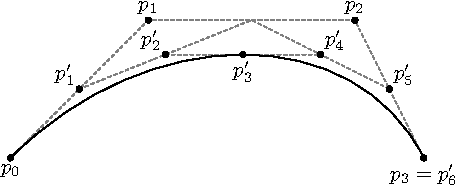
\includegraphics[scale=0.5]{subdivision}
    \caption[Subdivision of arc segments]{\footnotesize{Subdivision of arc segments. You can see that $ p_3 = p_6^\prime$.}} %the special ToC caption is in square brackets. The \footnotesize makes the figure caption smaller
    \label{barplot}
    \end{center}
    \end{figure} 

\chapter*{Conclusion}
         \addcontentsline{toc}{chapter}{Conclusion}
	\chaptermark{Conclusion}
	\markboth{Conclusion}{Conclusion}
	\setcounter{chapter}{4}
	\setcounter{section}{0}
	
Here's a conclusion, demonstrating the use of all that manual incrementing and table of contents adding that has to happen if you use the starred form of the chapter command. The deal is, the chapter command in \LaTeX\ does a lot of things: it increments the chapter counter, it resets the section counter to zero, it puts the name of the chapter into the table of contents and the running headers, and probably some other stuff. 

So, if you remove all that stuff because you don't like it to say ``Chapter 4: Conclusion'', then you have to manually add all the things \LaTeX\ would normally do for you. Maybe someday we'll write a new chapter macro that doesn't add ``Chapter X'' to the beginning of every chapter title.

\section{More info}
And here's some other random info: the first paragraph after a chapter title or section head \emph{shouldn't be} indented, because indents are to tell the reader that you're starting a new paragraph. Since that's obvious after a chapter or section title, proper typesetting doesn't add an indent there. 




%If you feel it necessary to include an appendix, it goes here.
    \appendix
      \chapter{The First Appendix}
      \chapter{The Second Appendix, for Fun}


%This is where endnotes are supposed to go, if you have them.
%I have no idea how endnotes work with LaTeX.

  \backmatter % backmatter makes the index and bibliography appear properly in the t.o.c...

% The next line forces every entry in your bibliography to be displayed, regardless of whether or not you've cited it in your thesis.
%    \nocite{*}

% For more details on customizing how your bibliography appears:
% https://www.overleaf.com/learn/latex/Bibliography_management_with_biblatex#Customizing_the_bibliography
\printbibliography[heading=bibintoc]

% Finally, an index would go here... but it is also optional.
\end{document}
